\chapter{Additional content}

\begin{table}[H]
    \centering
    \caption{Unilabs test catalog}
    \label{tab:test_catalog}
    \resizebox{0.7\textwidth}{!}{%
    \begin{tabular}{@{}l@{}}
    \toprule
    \multicolumn{1}{c}{\textbf{Test Catalog}}               \\ \midrule
    \ac{wes}                                                \\
    \acl{ngs}                                               \\
    Sanger Sequencing                                       \\
    \ac{acgh}                                               \\
    Karyotyping                                             \\
    \ac{fish}                                               \\
    QF-PCR, qPCR, RT-PCR                                    \\
    Fragment and Expansion Analysis                         \\
    \ac{mlpa}                                               \\
    Single Gene Analysis                                    \\
    Variant Analysis                                        \\
    Cytogenetics                                            \\
    NIPT | Tomorrow                                         \\ \bottomrule
    \end{tabular}
    }
\end{table}

\begin{table}[]
    \centering
    \caption{Samtools - BED file documentation}
    \label{tab:bed_file}
    \resizebox{0.8\textwidth}{!}{%
    \begin{tabular}{@{}rllll@{}}
    \toprule
    \textbf{Column} & \textbf{BED Field} & \textbf{Type} & \textbf{Regex or range}                                       & \textbf{Brief description} \\ \midrule
    1  & chrom      & String & {[}[a-zA-Z0-9\_]{1,255}{]}        & Chromosome name        \\
    2  & chromStart & Int    & {[}0, $2^{64}$ - 1{]}             & Feature start position \\
    3  & chromEnd   & Int    & {[}0, $2^{64}$ - 1{]}             & Feature end position   \\
    4  & name       & String & {[}\textbackslash x20-\textbackslash x7e{]}{1,255} & Feature description        \\
    5  & score      & Int    & {[}0, 1000{]}                     & A numerical value      \\
    6  & strand     & String & {[}-+.{]}                         & Feature strand         \\
    7  & thickStart & Int    & {[}0, $2^{64}$ - 1{]}             & Thick start position   \\
    8  & thickEnd   & Int    & {[}0, $2^{64}$ - 1{]}             & Thick end position     \\
    9  & itemRgb    & Int,Int,Int & ({[}0, 255{]}, {[}0, 255{]}, {[}0, 255{]}) | 0 & Display color \\
    10 & blockCount & Int    & {[}0, chromEnd - chromStart{]}    & Number of blocks       \\
    11 & blockSizes & List{[}Int{]} & ({[}[0-9]{]}+,){blockCount-1}{[}[0-9]{]}+,? & Block sizes \\
    12 & blockStarts & List{[}Int{]} & ({[}[0-9]{]}+,){blockCount-1}{[}[0-9]{]}+,? & Block start positions \\ \bottomrule
    \end{tabular}
    }
\end{table}

    
\begin{figure}[H]
    \centering
    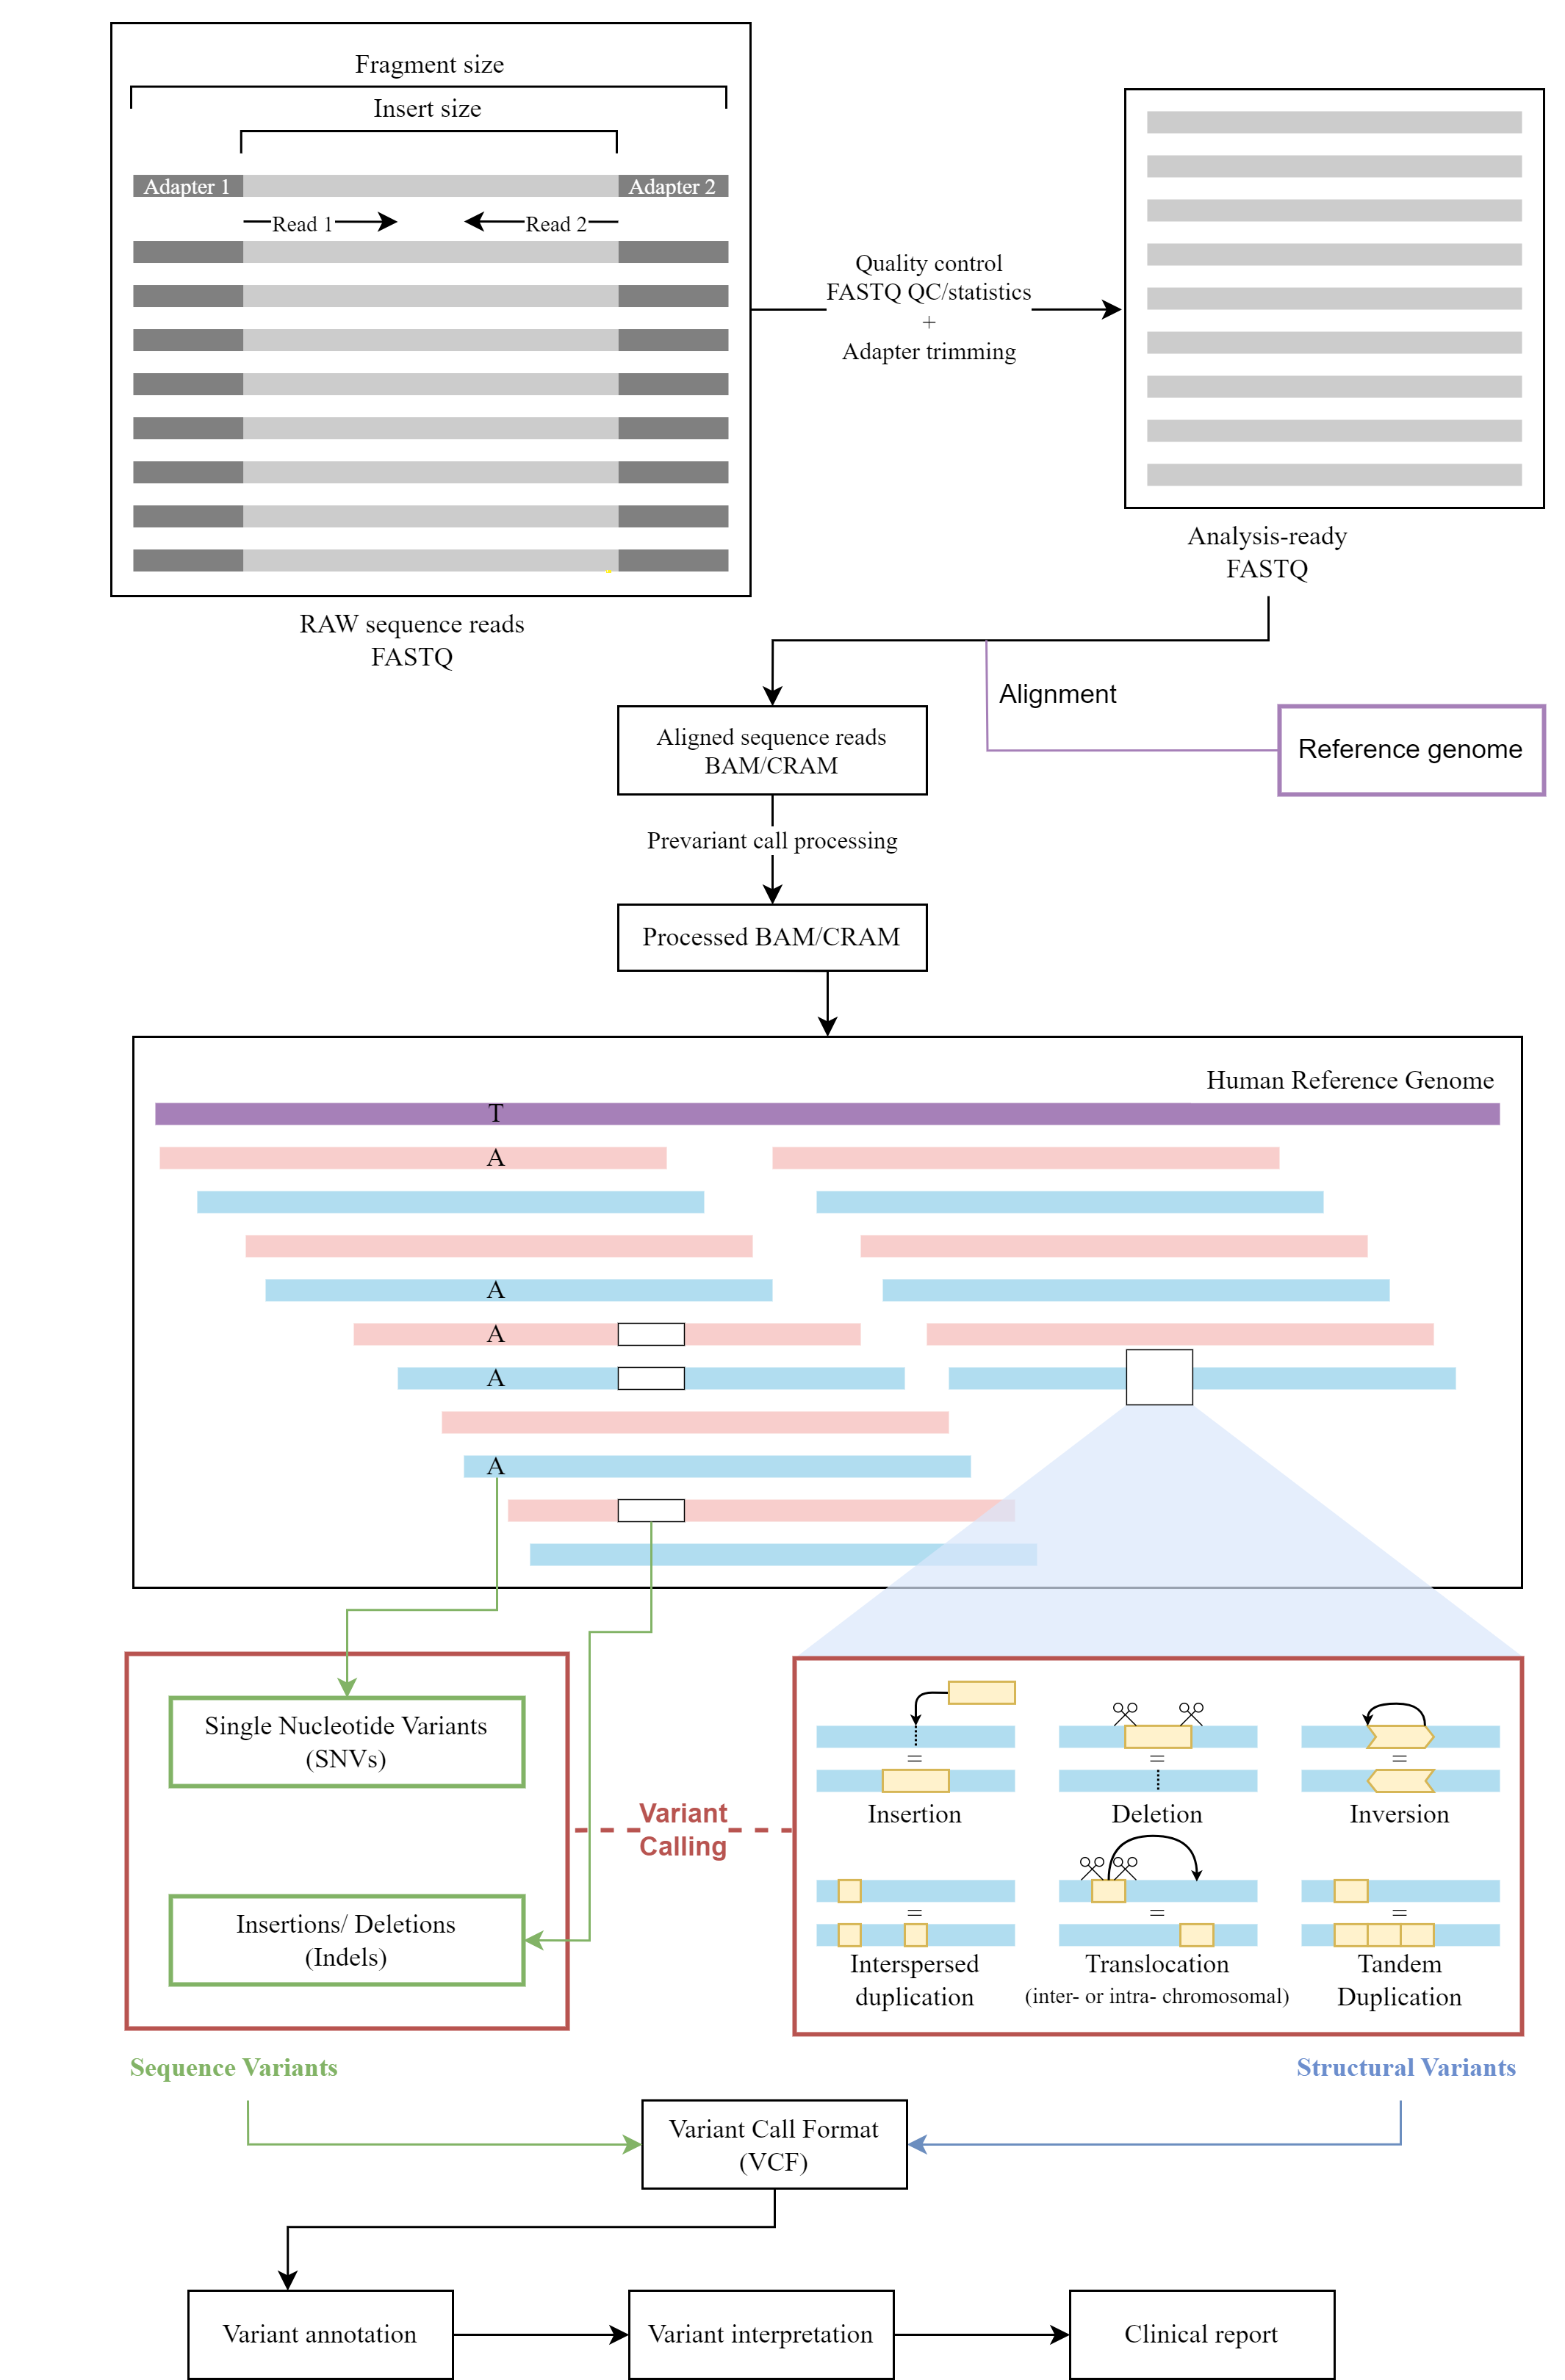
\includegraphics[width=0.9\textwidth]{figs/pipeline.png}
    \caption{NGS data analysis pipeline. Adapted from \cite{Roy2018}, \cite{pipeline}, \cite{Roy2020}, \cite{Kanzi2020}} 
    \label{fig:pipeline}
\end{figure}
